\documentclass{libs/XJTLU_format}
% \documentclass{beamer}
% Inserting the preamble file with the packages
\input{libs/preamble.tex}
\usepackage{booktabs}
\usepackage{adjustbox}
% Inserting the references file
\bibliography{references.bib}

% Title
\title[University of Liverpool Beamer Template]{\huge\textbf{March Report on FYP}}
% Subtitle
\subtitle{Machine Learning Assisted Real-time Diagnosis on CO2 Discharge Process}
% Author of the presentation
\author{Mingjie Zhu (Jay Zhu)}
% Institute's Name
\institute[University of Liverpool]{
    % email for contact
    \normalsize{\email{sgmzhu11@liverpool.ac.uk}}
    \newline
    % Department Name
    % University name
    \university{University of Liverpool}
}
% date of the presentation
\date{March 8, 2026}


%%%%%%%%%%%%%%%%%%%%%%%%%%%%%%%%%%%%%%%%%%%%%%%%%%%%%%%%%%%%%%%%%%%%%%%%%%%%%%%%%%
%% Start Document of the Presentation                                           %%
%%%%%%%%%%%%%%%%%%%%%%%%%%%%%%%%%%%%%%%%%%%%%%%%%%%%%%%%%%%%%%%%%%%%%%%%%%%%%%%%%%
\begin{document}
% insert the code style
\input{libs/code}

%% ---------------------------------------------------------------------------
% Title frame
\begin{frame}{}
    \maketitle
\end{frame}

%% ---------------------------------------------------------------------------
% Table of Contents
\begin{frame}{Table of Contents}
    \begin{multicols}{2}
        \tableofcontents
    \end{multicols}
\end{frame}


%%%%%%%%%%%%%%%%%%%%%%%%%%%%%%%%%%%%%%%%%%%%%%%%%%%%%%%%%%%%%%%%%%%%%%%%%%%%%%%%%%
\section{Project Overview}
%%%%%%%%%%%%%%%%%%%%%%%%%%%%%%%%%%%%%%%%%%%%%%%%%%%%%%%%%%%%%%%%%%%%%%%%%%%%%%%%%%

%% ---------------------------------------------------------------------------
\begin{frame}{Problem Statement}
    \begin{itemize}
        \item Nanosecond pulsed CO$_2$ discharge in water produces H$_2$O$_2$ --- a key oxidant for water treatment
        \item Optical Emission Spectroscopy (OES) captures real-time plasma spectra (200--900\,nm, 701 channels)
        \item \textbf{Goal:} Predict H$_2$O$_2$ yield rate from OES data and discharge parameters using machine learning 
        \textcolor{red}{\&\& conduct analysis on features' contribution and model performance}
        \item \textbf{Challenge:} Only 20 experimental samples available (small-sample regime)
    \end{itemize}
\end{frame}

%% ---------------------------------------------------------------------------
\begin{frame}{Project Phases}
    The project is conducted in 4 iterative phases, each building on the previous one to enhance model performance and interpretability:
    \begin{enumerate}
        \item \textbf{Phase 1:} Baseline modeling with PCA-reduced OES features + discharge parameters
        \item \textbf{Phase 2:} Hyperparameter tuning of nonlinear models (RF, MLP, CNN) using Bayesian optimization
        \item \textbf{Phase 3:} Domain-knowledge-driven manual feature engineering (13 physics-based OES features)
        \item \textbf{Phase 4:} Interpretability analysis and feature reduction via multi-model consensus and backward elimination
    \end{enumerate}
\end{frame}

%% ---------------------------------------------------------------------------
\begin{frame}{Experimental Data \& Configurations}
    \begin{table}[h]
        \centering
        \small
        \begin{tabular}{@{}clc@{}}
            \toprule
            \textbf{Config} & \textbf{Input Features} & \textbf{Dimensions} \\
            \midrule
            A & OES only (PCA-reduced) & 11 \\
            B & Discharge parameters only & 4 \\
            C & OES + discharge parameters & 15 (P1) / 17 (P3) \\
            \bottomrule
        \end{tabular}
    \end{table}
    \vspace{0.3em}
    \begin{itemize}
        \item \textbf{Discharge parameters:} frequency, pulse width, rise time, flow rate
        \item \textbf{Models tested:} Ridge, PLS, SVR, XGBoost, RF, MLP, CNN
        \item \textbf{Evaluation:} Leave-One-Out Cross-Validation (LOOCV) on 20 samples
        \item \textbf{Target:} H$_2$O$_2$ yield rate (range: 0.02--0.83)
    \end{itemize}
\end{frame}


%%%%%%%%%%%%%%%%%%%%%%%%%%%%%%%%%%%%%%%%%%%%%%%%%%%%%%%%%%%%%%%%%%%%%%%%%%%%%%%%%%
\section{Phase 1: Baseline Modeling with PCA}
%%%%%%%%%%%%%%%%%%%%%%%%%%%%%%%%%%%%%%%%%%%%%%%%%%%%%%%%%%%%%%%%%%%%%%%%%%%%%%%%%%

%% ---------------------------------------------------------------------------
\begin{frame}{Phase 1: PCA Dimensionality Reduction}
    \begin{columns}
        \begin{column}{0.55\textwidth}
            \begin{itemize}
                \item 701-channel OES spectrum reduced via PCA
                \item 11 principal components retained (95\% cumulative variance)
                \item Severe curse of dimensionality: $p/n$ ratio too high for 20 samples
            \end{itemize}
        \end{column}
        \begin{column}{0.45\textwidth}
            \begin{figure}
                \centering
                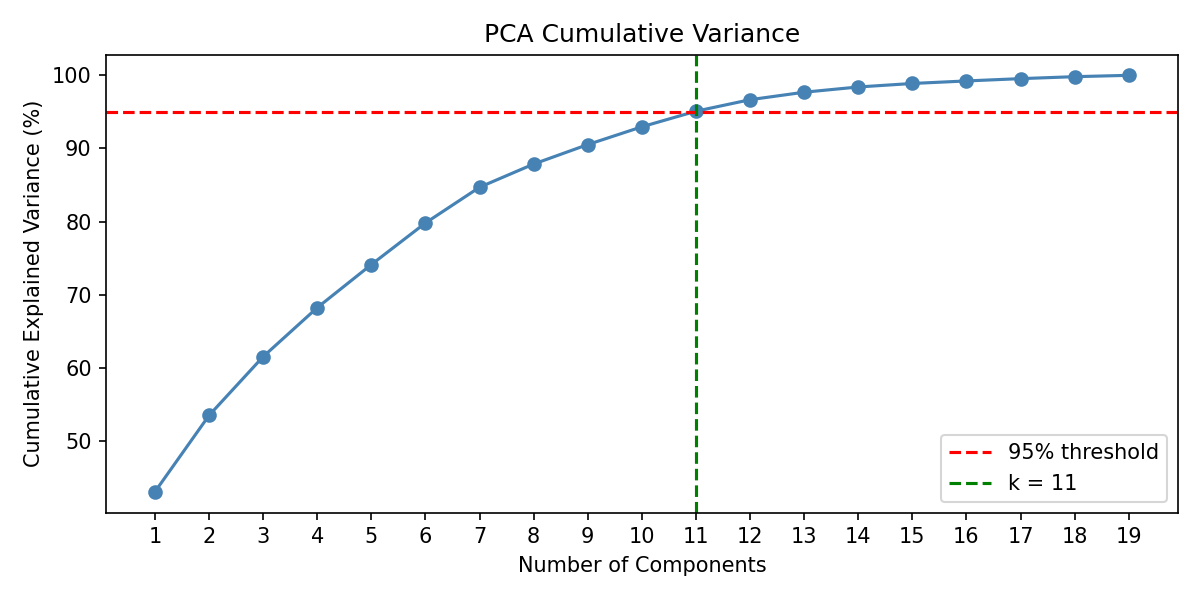
\includegraphics[width=\textwidth]{image/pca_cumulative_variance.png}
            \end{figure}
        \end{column}
    \end{columns}
\end{frame}

%% ---------------------------------------------------------------------------
\begin{frame}{Phase 1: Results --- R$^2$ Heatmap (7 Models $\times$ 3 Configs)}
    \begin{figure}
        \centering
        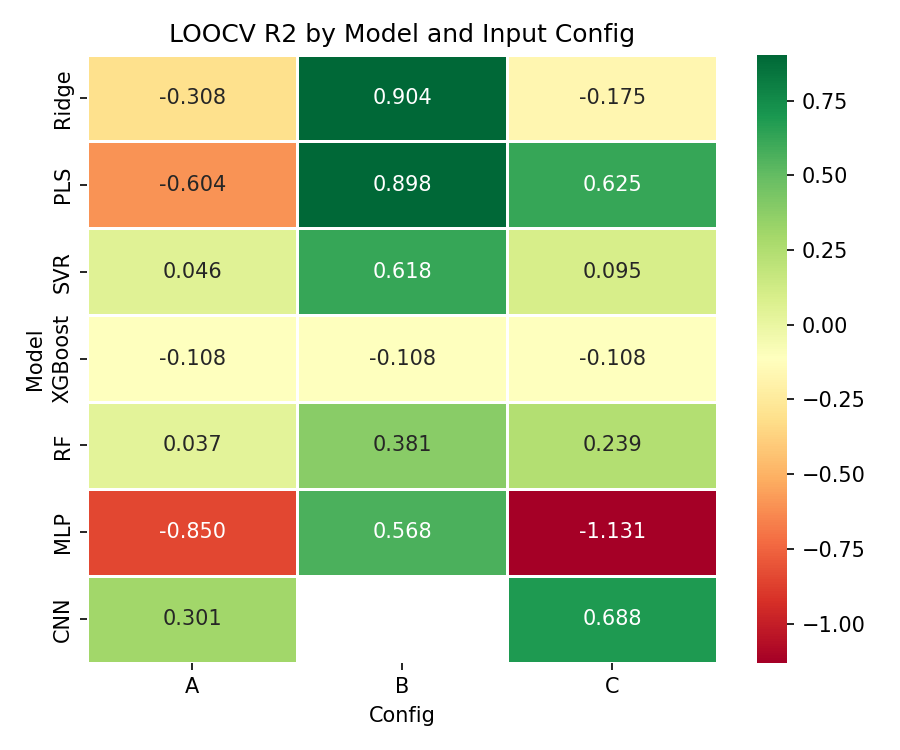
\includegraphics[width=0.5\textwidth]{image/heatmap_R2.png}
    \end{figure}
    \begin{itemize}
        \item \textbf{Best:} Ridge Config B achieved R$^2$ = 0.90 (discharge params only)
        \item \textcolor{red}{Discharge-parameter-only models (config B) outperformed OES-only (config A) and combined (config C) models}
    \end{itemize}
\end{frame}


%%%%%%%%%%%%%%%%%%%%%%%%%%%%%%%%%%%%%%%%%%%%%%%%%%%%%%%%%%%%%%%%%%%%%%%%%%%%%%%%%%
\section{Phase 2: Hyperparameter Tuning}
%%%%%%%%%%%%%%%%%%%%%%%%%%%%%%%%%%%%%%%%%%%%%%%%%%%%%%%%%%%%%%%%%%%%%%%%%%%%%%%%%%
\begin{frame}{Phase 2: Motivation for Hyperparameter Tuning}
    \begin{itemize}
        \item Phase 1 used default hyperparameters, which may not suit our small-sample, high-dimensional data
        \item Nonlinear models (RF, MLP, CNN) showed potential but **underperformed** due to either suboptimal settings or limited data
        \item Bayesian optimization can efficiently explore the hyperparameter space to enhance model performance. Thus can potentially recover nonlinear models' performance and better leverage OES features, especially in Config C
    \end{itemize}
    
\end{frame}

%% ---------------------------------------------------------------------------
\begin{frame}{Phase 2: Bayesian Optimization}
    \begin{itemize}
        \item Applied \textbf{Optuna} (TPE sampler) with nested LOOCV
        \item Tuned RF, MLP, and CNN: 100--200 trials per model-config pair
        \item Goal: recover nonlinear models from poor Phase~1 defaults
    \end{itemize}
    \vspace{0.5em}
    Key improvements after tuning:
    \begin{table}[h]
        \centering
        \small
        \begin{tabular}{@{}llccc@{}}
            \toprule
            \textbf{Model} & \textbf{Config} & \textbf{R$^2$ (P1)} & \textbf{R$^2$ (P2)} & \textbf{$\Delta$R$^2$} \\
            \midrule
            MLP & \textcolor{red}{C} & $-1.13$ & 0.37 & \textcolor{red}{$+1.50$} \\
            MLP & A & $-0.85$ & 0.37 & $+1.22$ \\
            RF  & B & 0.38 & 0.75 & $+0.37$ \\
            MLP & \textcolor{red}{B} & 0.57 & \textcolor{red}{0.86} & $+0.29$ \\
            CNN & \textcolor{red}{C} & 0.69 & \textcolor{red}{0.77} & $+0.09$ \\
            \bottomrule
        \end{tabular}
    \end{table}
\end{frame}

%% ---------------------------------------------------------------------------
\begin{frame}{Phase 2: Results --- Phase 1 vs Phase 2 Comparison}
    \begin{figure}
        \centering
        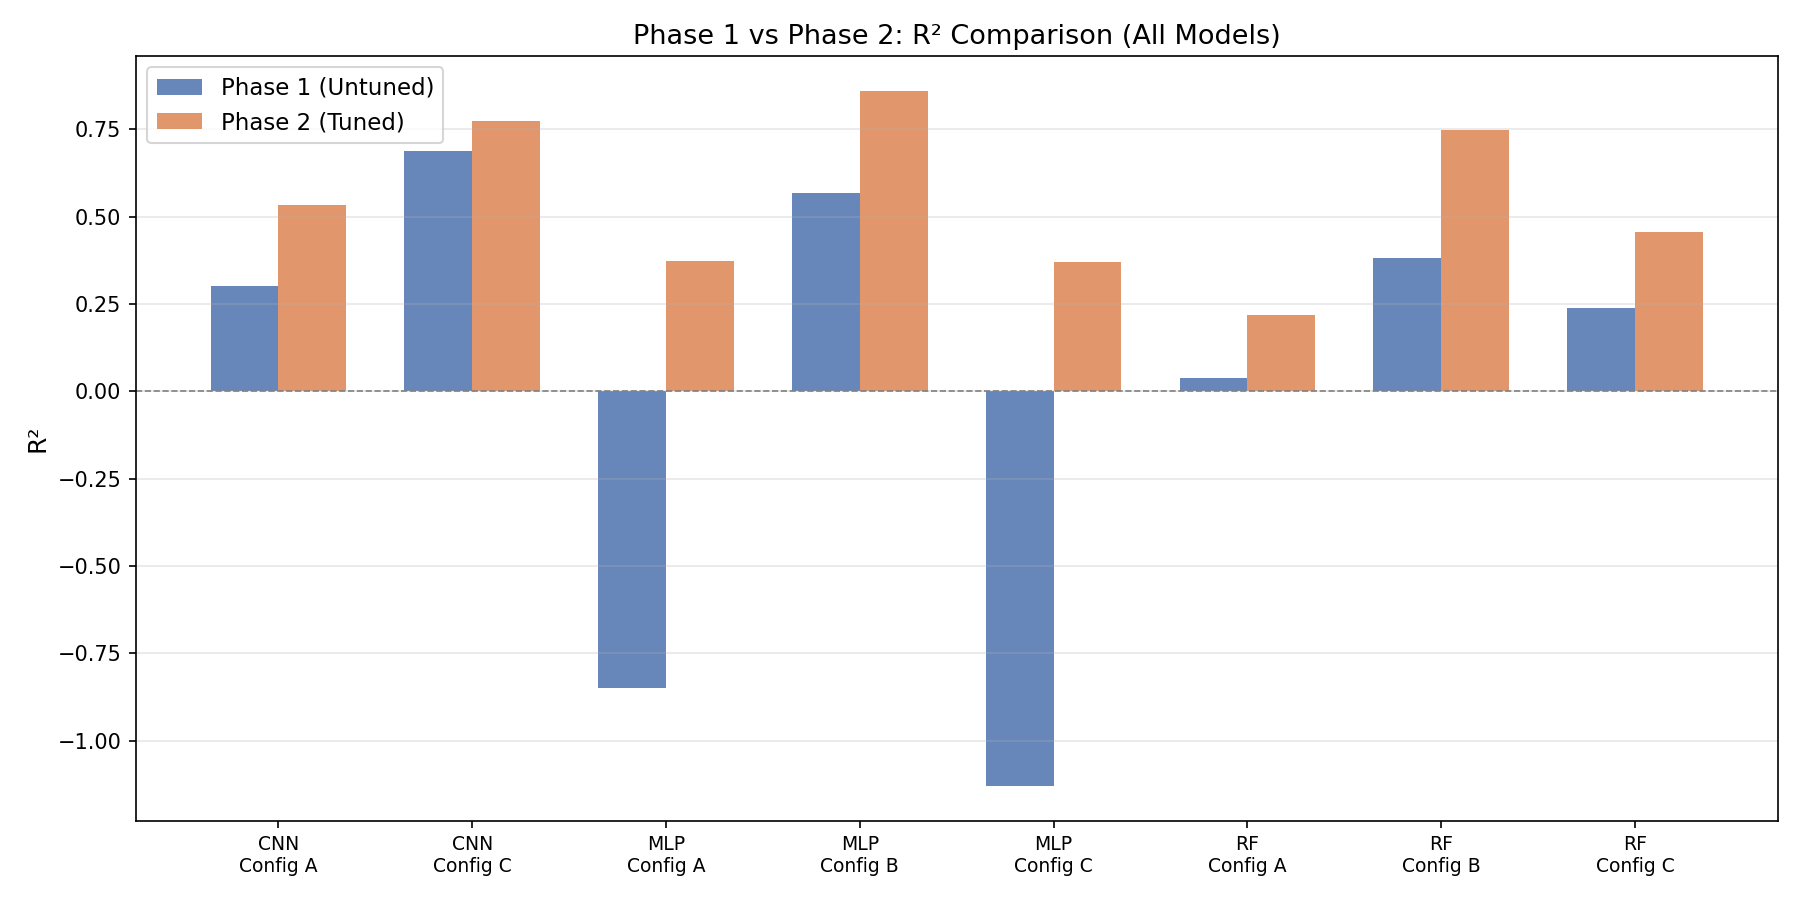
\includegraphics[width=0.75\textwidth]{image/phase1_vs_phase2_comparison.png}
    \end{figure}
    \begin{itemize}
        \item Tuning universally beneficial, improving the non-linear ML models (MLP, RF, CNN) across all configs
        \item But Config B still dominant, and OES features via PCA remained weak even with optimized models
    \end{itemize}
\end{frame}


%%%%%%%%%%%%%%%%%%%%%%%%%%%%%%%%%%%%%%%%%%%%%%%%%%%%%%%%%%%%%%%%%%%%%%%%%%%%%%%%%%
\section{Phase 3: Domain-Knowledge Feature Engineering}
%%%%%%%%%%%%%%%%%%%%%%%%%%%%%%%%%%%%%%%%%%%%%%%%%%%%%%%%%%%%%%%%%%%%%%%%%%%%%%%%%%

\begin{frame}{Phase 3: Motivation for Domain-Knowledge Feature Engineering}
    \begin{itemize}
        \item PCA features are abstract, it only shows variance but lacks physical meaning, and may not capture the underlying plasma chemistry relevant to H$_2$O$_2$ production
        \item Leveraging domain knowledge (plasma chemistry) to engineer specific OES features (e.g., intensities of key emission lines, band integrals, ratios) can create more meaningful inputs that directly relate to chemical processes
        \item Hypothesis: Higher representative Physics-based features will enhance model interpretability and predictive power, especially in Config C where OES data is combined with discharge parameters
    \end{itemize}
    
\end{frame}

%% ---------------------------------------------------------------------------
\begin{frame}{Phase 3: 13 Physics-Based OES Features}
    Replaced blind PCA with features grounded in plasma chemistry:
    \vspace{0.3em}
    \begin{adjustbox}{max width=\textwidth}
    \small
    \begin{tabular}{@{}cllll@{}}
        \toprule
        \textbf{ID} & \textbf{Feature} & \textbf{Type} & \textbf{Species} & \textbf{Role} \\
        \midrule
        F1  & I(309\,nm)        & Intensity & OH        & Direct H$_2$O$_2$ precursor \\
        F2  & I(777\,nm)        & Intensity & O atom    & CO$_2$ dissociation product \\
        F3  & I(656\,nm)        & Intensity & H$\alpha$ & H$_2$O dissociation degree \\
        F4  & I(486\,nm)        & Intensity & H$\beta$  & H$_2$O dissociation degree \\
        F5  & I(337\,nm)        & Intensity & N$_2$ SPS & High-energy $e^-$ marker$^{[2]}$ \\
        F6  & I(406\,nm)        & Intensity & CO$_2^+$  & CO$_2$ ionization degree \\
        F7  & I(516\,nm)        & Intensity & C$_2$     & Possible Deep decomposition \\
        \midrule
        F8  & $\int$(306--312)   & Band integral & OH 0-0 band    & Robust OH emission \\
        F9  & $\int$(398--412)   & Band integral & CO$_2^+$ FDB   & Aggregate ionization \\
        F10 & $\int$(460--500)   & Band integral & CO + H$\beta$  & CO + H$_2$O dissociation \\
        \midrule
        F11 & I(309)/I(656)     & Ratio & OH/H$\alpha$           & Relative OH availability \\
        F12 & I(777)/I(309)     & Ratio & O/OH                   & Relative OH availability \\
        F13 & I(656)/I(486)     & Ratio & H$\alpha$/H$\beta$     & Balmer decrement - e$^-$ marker$^{[3]}$ \\
        \bottomrule
    \end{tabular}
    \end{adjustbox}
\end{frame}

%% ---------------------------------------------------------------------------
\begin{frame}{Phase 3: \textcolor{red}{Significant} Results --- Cross-Phase Comparison}
    \begin{figure}
        \centering
        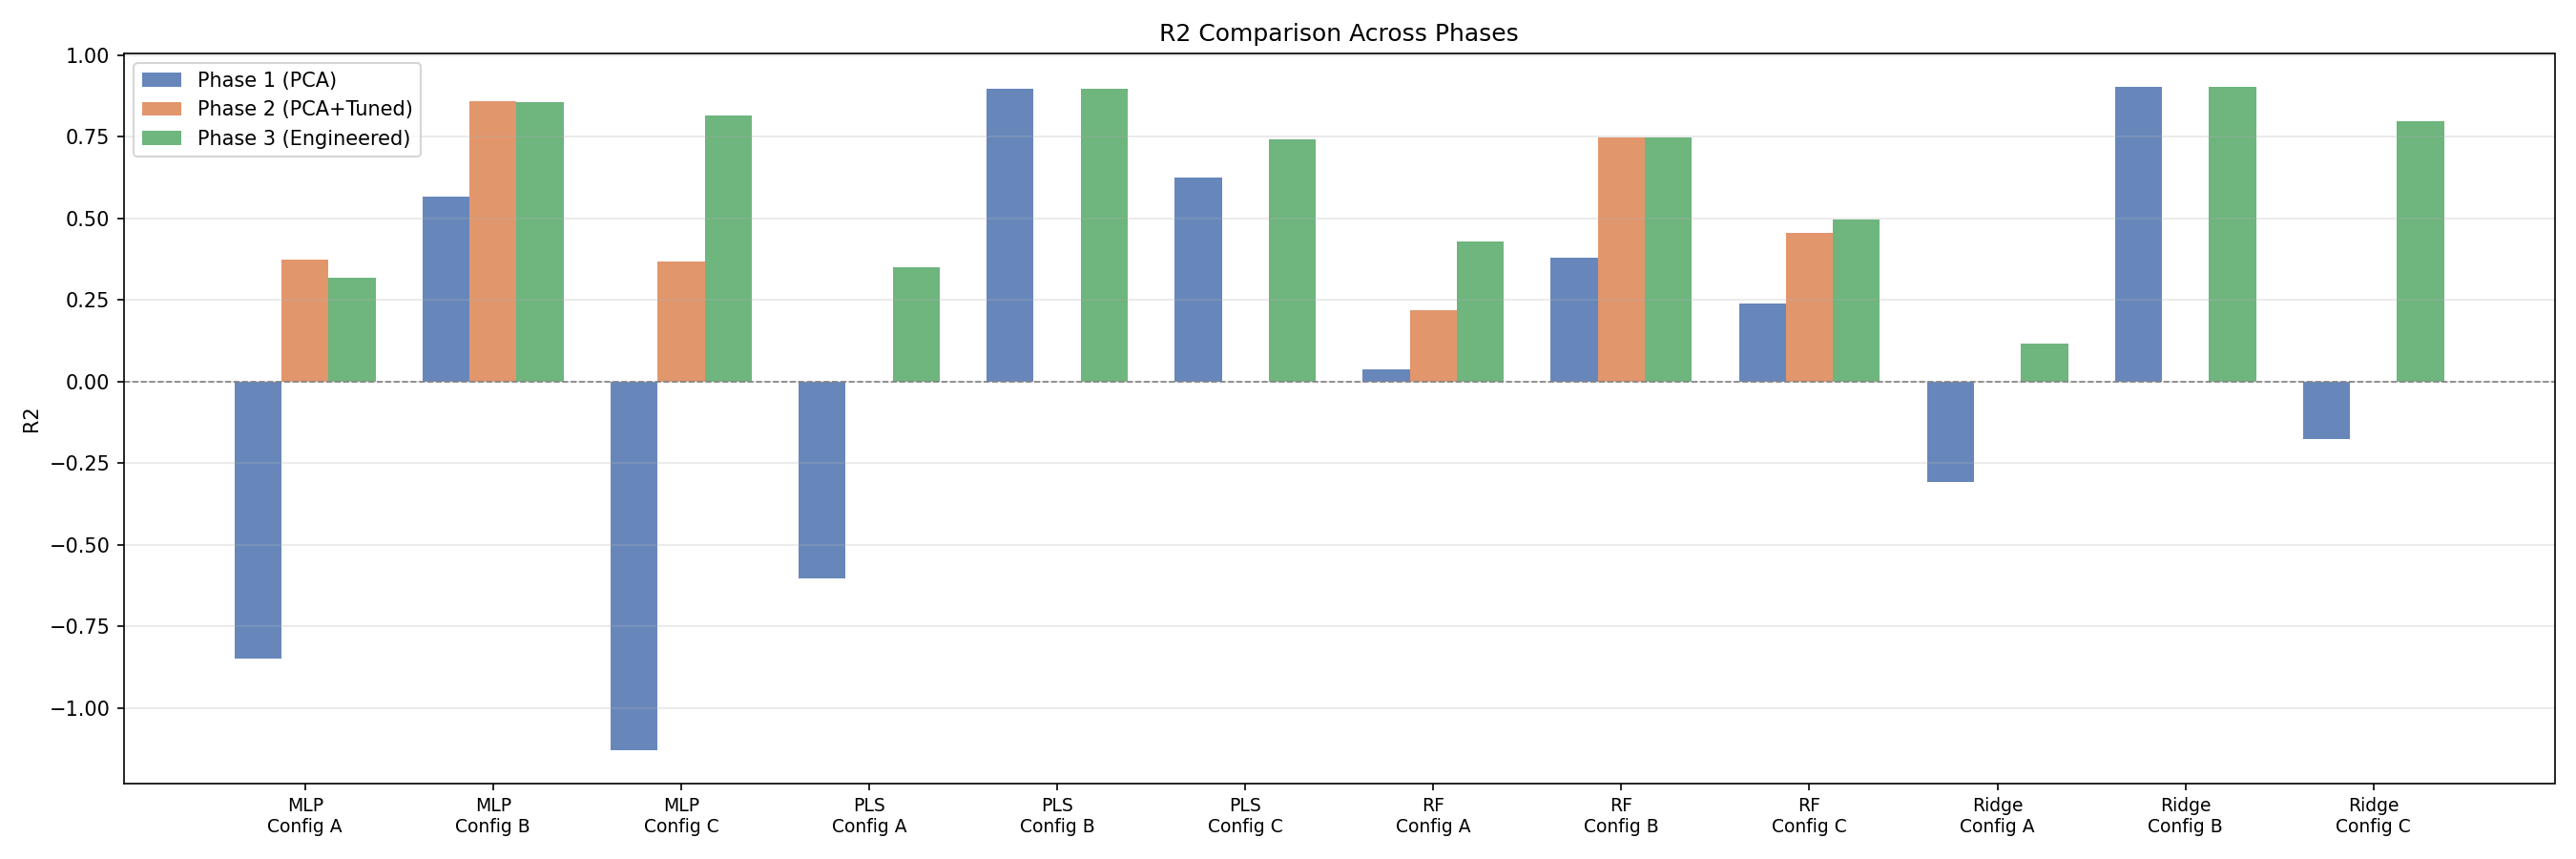
\includegraphics[width=\textwidth]{image/phase1_vs_phase3_comparison.png}
    \end{figure}
    \begin{itemize}
        \item \textbf{Ridge Config C:} R$^2$ improved from $-0.17$ to $0.80$ ($+0.97$)
        \item \textbf{MLP Config C:} R$^2$ improved from $-1.13$ to $0.82$ ($+1.95$)
        \item \textcolor{red}{Domain knowledge dramatically unlocked OES predictive power}
    \end{itemize}
\end{frame}


%%%%%%%%%%%%%%%%%%%%%%%%%%%%%%%%%%%%%%%%%%%%%%%%%%%%%%%%%%%%%%%%%%%%%%%%%%%%%%%%%%
\section{Phase 4: Interpretability \& Feature Reduction}
%%%%%%%%%%%%%%%%%%%%%%%%%%%%%%%%%%%%%%%%%%%%%%%%%%%%%%%%%%%%%%%%%%%%%%%%%%%%%%%%%%
\begin{frame}{Phase 4: Motivation for Interpretability and Feature Reduction}
    \begin{itemize}
        \item Phase 3's physics-based features improved performance but increased model complexity (17 features), risking overfitting in our small-sample regime
        \item Understanding which features are most influential can enhance interpretability, avoid overfitting and probably improve generalization by removing redundant or noisy features (feature work)
        \item Hypothesis: A smaller subset of the most important features (e.g., top 5-7) can achieve comparable or better performance than the full set by reducing collinearity and noise, while also providing clearer insights into the key plasma processes driving H$_2$O$_2$ production
    \end{itemize}
    
\end{frame}

%% ---------------------------------------------------------------------------
\begin{frame}{Phase 4: Multi-Model Feature Importance Consensus}
    \begin{figure}
        \centering
        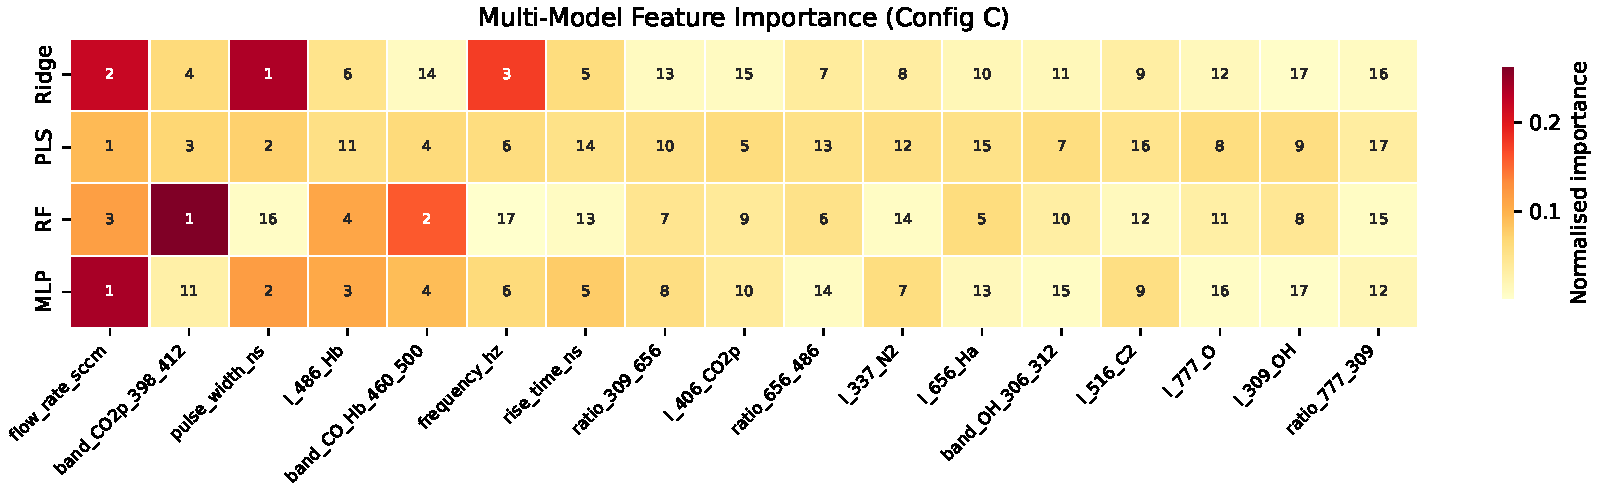
\includegraphics[width=\textwidth]{image/feature_importance_heatmap.pdf}
    \end{figure}
    \begin{itemize}
        \item Ranked 17 features across Ridge, PLS, RF, and MLP (SHAP)
        \item \textbf{Top/Significant features:} flow rate, CO$_2^+$ band integral, pulse width
    \end{itemize}
\end{frame}

% %% ---------------------------------------------------------------------------
% \begin{frame}{Phase 4: Backward Elimination --- Ablation Trajectory}
%     \begin{figure}
%         \centering
%         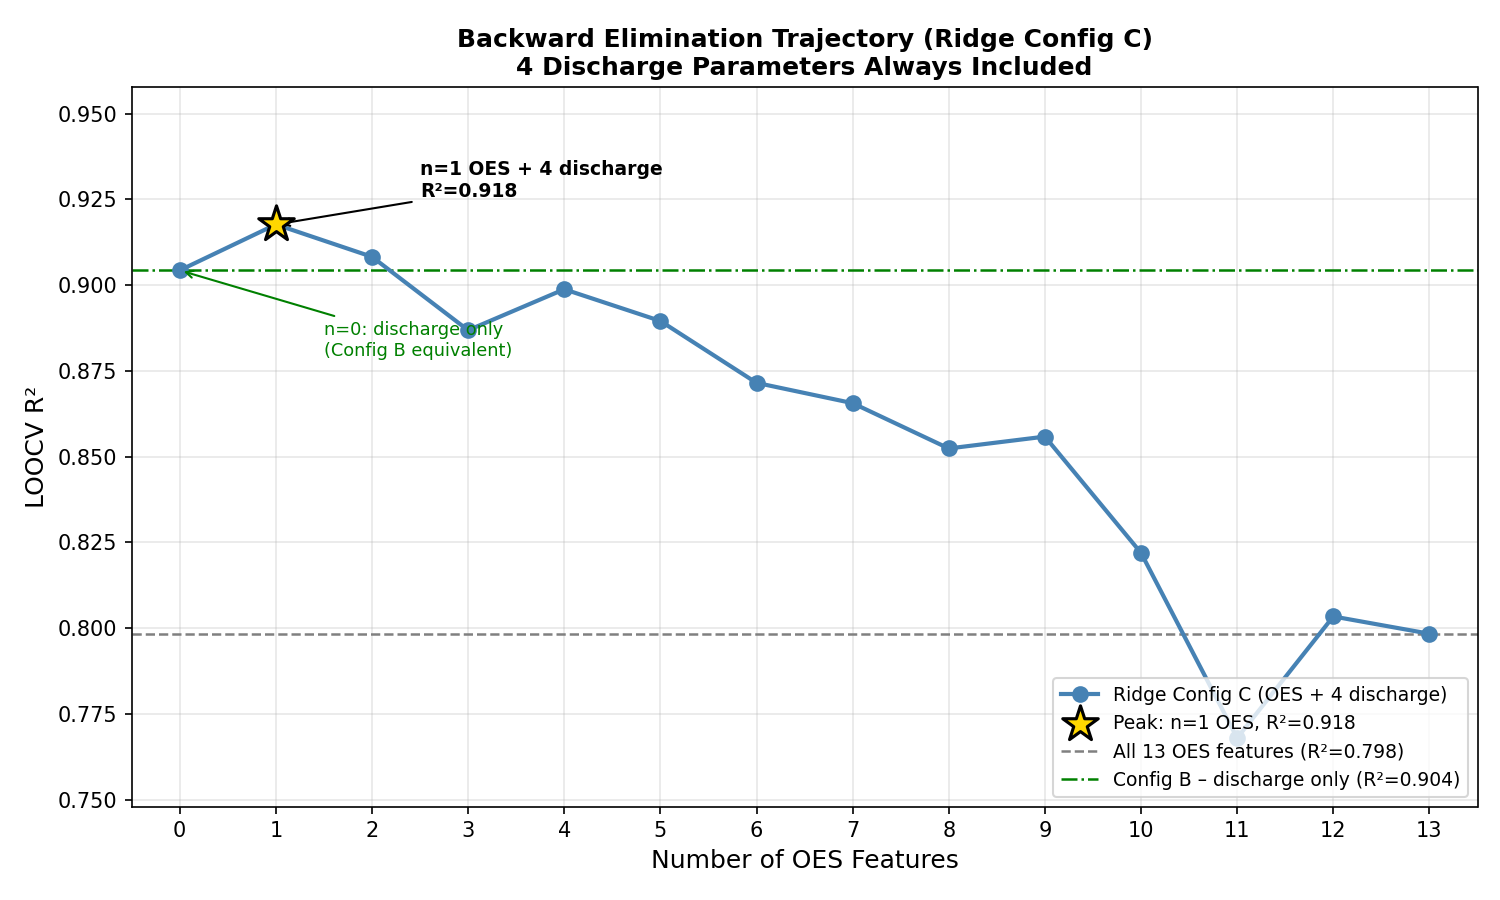
\includegraphics[width=0.75\textwidth]{image/ablation_trajectory.png}
%     \end{figure}
%     \begin{itemize}
%         \item Removing redundant OES features \textbf{improves} R$^2$ (collinearity reduction)
%         \item Optimal: \textbf{4 OES + 4 discharge params} $\rightarrow$ R$^2$ = 0.899
%         \item Category ablation: 3 ratios alone + 4 params $\rightarrow$ R$^2$ = 0.920
%     \end{itemize}
% \end{frame}

%% ---------------------------------------------------------------------------
\begin{frame}{Phase 4: Statistical Validation}
    \begin{columns}
        \begin{column}{0.55\textwidth}
            \begin{figure}
                \centering
                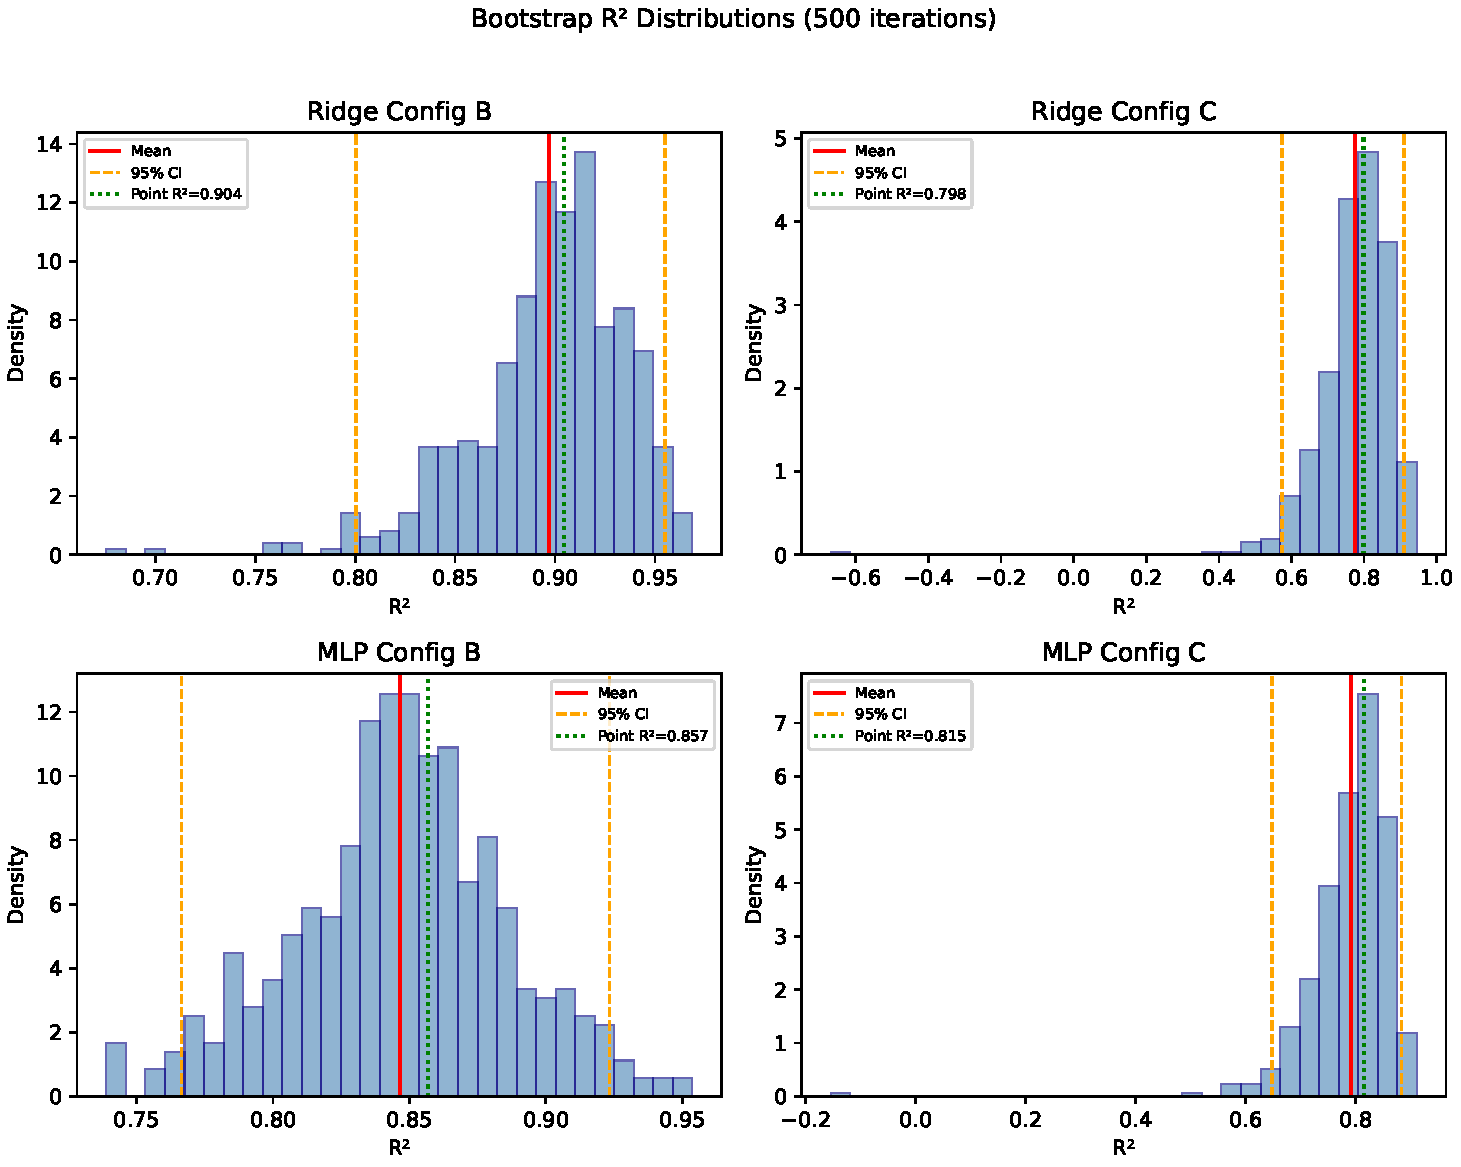
\includegraphics[width=\textwidth]{image/bootstrap_r2.pdf}
            \end{figure}
        \end{column}
        \begin{column}{0.45\textwidth}
            \textbf{Bootstrap 95\% CIs} (500 resamples):
            \vspace{0.3em}
            \small
            \begin{tabular}{@{}lc@{}}
                \toprule
                \textbf{Model} & \textbf{R$^2$ [95\% CI]} \\
                \midrule
                Ridge B & 0.90 [0.80, 0.95] \\
                Ridge C & 0.80 [0.57, 0.91] \\
                MLP C   & 0.82 [0.65, 0.88] \\
                MLP B   & 0.86 [0.77, 0.92] \\
                \bottomrule
            \end{tabular}
            \vspace{0.5em}

            \textbf{Permutation test} (2000 iter.):
            \begin{itemize}
                \item Observed R$^2$ = 0.920
                \item $p < 0.0005$
            \end{itemize}
        \end{column}
    \end{columns}

    \begin{itemize}
        \item Ridge and MLP Config C are statistically indistinguishable
    \end{itemize}
\end{frame}

%% ---------------------------------------------------------------------------
\begin{frame}{Phase 4: Final Optimized Model}
    \begin{table}[h]
        \centering
        \begin{tabular}{@{}ll@{}}
            \toprule
            \textbf{Property} & \textbf{Value} \\
            \midrule
            Model & Ridge Regression \\
            Total features & 7 \\
            OES features (3) & I(309)/I(656), I(777)/I(309), I(656)/I(486) \\
            Discharge params (4) & frequency, pulse width, rise time, flow rate \\
            R$^2$ (LOOCV) & \textbf{0.920} \\
            Permutation $p$-value & $< 0.0005$ \\
            \bottomrule
        \end{tabular}
    \end{table}
    \vspace{0.5em}
    \begin{itemize}
        \item 3 OES intensity ratios + 4 discharge parameters = \textbf{7 features total}
        \item Outperforms the full 17-feature model (R$^2$ = 0.798) by removing collinear noise
        \item Simple, interpretable, and statistically significant
    \end{itemize}
\end{frame}


%%%%%%%%%%%%%%%%%%%%%%%%%%%%%%%%%%%%%%%%%%%%%%%%%%%%%%%%%%%%%%%%%%%%%%%%%%%%%%%%%%
\section{Summary}
%%%%%%%%%%%%%%%%%%%%%%%%%%%%%%%%%%%%%%%%%%%%%%%%%%%%%%%%%%%%%%%%%%%%%%%%%%%%%%%%%%

%% ---------------------------------------------------------------------------
\begin{frame}{Progress Summary: R$^2$ Evolution Across Phases}
    \begin{table}[h]
        \centering
        \begin{tabular}{@{}clccp{4.5cm}@{}}
            \toprule
            \textbf{Phase} & \textbf{Best Model} & \textbf{Config} & \textbf{R$^2$} & \textbf{Key Advancement} \\
            \midrule
            1 & Ridge & B & 0.904 & Baseline; PCA for OES failed \\
            2 & MLP   & B & 0.861 & Bayesian hyperparameter tuning \\
            3 & MLP   & C & 0.815 & Domain-knowledge OES features \\
            4 & Ridge & C (pruned) & \textbf{0.920} & Feature reduction + interpretability \\
            \bottomrule
        \end{tabular}
    \end{table}
    \vspace{0.5em}

\end{frame}

%% ---------------------------------------------------------------------------
\begin{frame}{Conclusion}
    \textbf{Progress Summary}
    \begin{itemize}
        \item Successfully developed a machine learning model to predict H$_2$O$_2$ yield from OES and discharge parameters 
        \item Demonstrated the critical importance of domain-knowledge-driven feature engineering in unlocking OES predictive power
        \item Identified key features that drive model performance best, enhancing interpretability and reducing overfitting risk
    \end{itemize}

    \textbf{Findings}
    \begin{itemize}
        \item Domain knowledge + feature reduction outperformed complex models on small data
        \item OES features became useful only after physics-guided engineering (Phase 3)
        \item Final model: simple Ridge with 7 features achieves R$^2$ = 0.920 ($p < 0.0005$)
    \end{itemize}
\end{frame}



% %% ---------------------------------------------------------------------------
% % Reference frames
% \begin{frame}[allowframebreaks]
%     \frametitle{Reference}
%         \tiny\printbibliography
% \end{frame}

%% ---------------------------------------------------------------------------
% Final frame
\begin{frame}{}
    \centering
    \huge{\textbf{\example{Thank You !}}}

\end{frame}

\end{document}
